        %%******************************************%%
        %%                                          %%
        %%        Modello di tesi di laurea         %%
        %%            di Andrea Giraldin            %%
        %%                                          %%
        %%             2 novembre 2012              %%
        %%                                          %%
        %%******************************************%%

\begin{document}
    \frontmatter
    \begin{titlepage}
    \begin{center}
        \begin{LARGE}
            \textbf{\myUni}\\
        \end{LARGE}

        \vspace{10pt}

        \begin{Large}
            \textsc{\myDepartment}\\
        \end{Large}

        \vspace{10pt}

        \begin{large}
            \textsc{\myFaculty}\\
        \end{large}

        \vspace{30pt}
        \begin{figure}[htbp]
            \centering
            
\includegraphics[height=6cm]{unipd-logo}
        \end{figure}
        \vspace{30pt}

        \begin{LARGE}
            \textbf{\myTitle}\\
        \end{LARGE}

        \vspace{10pt}

        \begin{large}
            \textsl{\myDegree}\\
        \end{large}

        \vspace{40pt}

        \begin{large}
            \begin{flushleft}
                \textit{Relatore}\\
                \vspace{5pt}
                \profTitle\ \myProf
            \end{flushleft}

            % You can tweak the spacing to have professor and student names on the same line
            % useful if the page is broken by a long thesis title and you need more space
            % \vspace{-52pt}

            \begin{flushright}
                \textit{Laureando}\\
                \vspace{5pt}
                \myName \\
                \vspace{5pt}
                \textit{Matricola} \myID
            \end{flushright}
        \end{large}

        \vspace{40pt}

        \line(1, 0){338} \\
        \begin{normalsize}
            \textsc{Anno Accademico \myAA}
        \end{normalsize}
    \end{center}
\end{titlepage}

    \clearpage
\phantomsection
\thispagestyle{empty}

\hfill
\vfill

\noindent\myName: \textit{\myTitle,}
\myDegree,
\textcopyright\ \myTime.

    \cleardoublepage
\phantomsection
\thispagestyle{empty}
\pdfbookmark{Dedica}{Dedica}

\vspace*{3cm}

\begin{center}
    Lorem ipsum dolor sit amet, consectetuer adipiscing elit. \\ \medskip
    --- Oscar Wilde
\end{center}

\medskip

\begin{center}
    Dedicato a ...
\end{center}

    \cleardoublepage
\phantomsection
\pdfbookmark{Sommario}{Sommario}
\begingroup
\let\clearpage\relax
\let\cleardoublepage\relax
\let\cleardoublepage\relax

\chapter*{Sommario}

Questo elaborato descrive l’attività svolta da Stefani Riccardo durante un tirocinio curriculare della durata di 320 ore presso l’azienda Oribea AI S.r.l.

Il progetto si inserisce negli ambiti della Business Intelligence e del Machine Learning, con l'obiettivo di sviluppare una Task AI per l'analisi delle vendite, utilizzando dati provenienti da database aziendali o dataset pubblici. Il sistema realizzato sfrutta un Large Language Model (LLM) per generare analisi automatiche, interpretabili e personalizzabili.

Inoltre, il progetto prevede anche lo sviluppo di un sistema di raccomandazione integrato in un'apposita Task AI, che permetta di raccomandare prodotti ai clienti in base alle loro preferenze e comportamenti di acquisto, e viceversa di suggerire possibili clienti a cui proporre i prodotti, ottimizzando le strategie di marketing e vendita.

Prima della fase di sviluppo, è stato condotto uno studio approfondito delle tecnologie impiegate e dei concetti economici fondamentali per garantire la qualità delle analisi delle vendite e delle raccomandazioni prodotte. Le attività e le soluzioni adottate vengono illustrate nei capitoli successivi.

%\vfill

%\selectlanguage{english}
%\pdfbookmark{Abstract}{Abstract}
%\chapter*{Abstract}

%\selectlanguage{italian}

\endgroup

\vfill

    \cleardoublepage
\phantomsection
\pdfbookmark{Ringraziamenti}{ringraziamenti}

\begin{flushright}{
    \slshape
    ``La differenza tra una persona di successo e gli altri non è la mancanza di forza, né la mancanza di conoscenza, ma piuttosto la mancanza di volontà.''} \\
    \medskip
    --- Vince Lombardi
\end{flushright}


\bigskip

\begingroup
\let\clearpage\relax
\let\cleardoublepage\relax
\let\cleardoublepage\relax

\chapter*{Ringraziamenti}

\noindent \textit{Innanzitutto, vorrei esprimere la mia gratitudine al Prof. \myProf, relatore della mia tesi, per l'aiuto e il sostegno fornitomi durante la stesura del lavoro.}\\

\noindent \textit{Desidero ringraziare con affetto i miei genitori per il sostegno, il grande aiuto e per essermi stati vicini in ogni momento durante gli anni di studio.}\\

\noindent \textit{Ho desiderio di ringraziare poi i miei amici per tutti i bellissimi anni passati insieme e le mille avventure vissute.}\\
\bigskip

\noindent\textit{\myLocation, \myTime}
\hfill \myName

\endgroup

    \cleardoublepage
\pdfbookmark{\contentsname}{tableofcontents}
\setcounter{tocdepth}{2}
\tableofcontents
%\markboth{\contentsname}{\contentsname}
\clearpage

\begingroup
    \let\clearpage\relax
    \let\cleardoublepage\relax
    \let\cleardoublepage\relax

    % Figures list
    \phantomsection
    \pdfbookmark{\listfigurename}{lof}
    \listoffigures

    \vspace*{8ex}

    % Tables list
    \phantomsection
    \pdfbookmark{\listtablename}{lot}
    \listoftables

    \vspace*{8ex}
\endgroup

\cleardoublepage

    \cleardoublepage

    \mainmatter
    \chapter{Introduzione}
\label{cap:introduzione}

\intro{In questo capitolo verrà descritta l’azienda proponente del tirocinio, il way of working, l’organizzazione del testo e delle convenzioni tipografiche impostate.}\\

\noindent Introduzione al contesto applicativo.\\

\noindent Esempio di utilizzo di un termine nel glossario \\
\gls{api}. \\

\noindent Esempio di citazione in linea \\
\cite{site:agile-manifesto}. \\

\noindent Esempio di citazione nel pie' di pagina \\
citazione\footcite{womak:lean-thinking} \\

\section{L'azienda}

Oribea AI S.r.l. è una startup innovativa fondata nel 2024 nella Repubblica di San Marino, in seguito alla separazione dall'azienda di e-commerce ITTweb. La missione di Oribea è fornire soluzioni avanzate di intelligenza artificiale per migliorare l'efficienza e la produttività delle aziende, con un focus particolare sull'implementazione di Large Language Models (LLM) e agenti intelligenti.
Tra i principali prodotti sviluppati da Oribea vi è l'AI Agent Builder, uno strumento che consente alle imprese di creare e integrare agenti intelligenti personalizzati nei propri processi aziendali. Questi agenti sono progettati per automatizzare attività ripetitive, migliorare la comunicazione interna ed esterna e supportare la presa di decisioni attraverso l'analisi avanzata dei dati. L'AI Agent Builder si distingue per la sua capacità di adattarsi alle specifiche esigenze di ciascuna azienda, offrendo soluzioni su misura che sfruttano le potenzialità degli LLM.
Inoltre, Oribea sta sviluppando un Sistema Intelligente, concepito per fungere da piattaforma centrale nell'orchestrazione delle attività aziendali. Questo sistema mira a integrare diverse applicazioni e servizi, facilitando la gestione dei processi e migliorando la coerenza e l'efficienza operativa. Attraverso l'uso di tecnologie avanzate di intelligenza artificiale, il Sistema Intelligente di Oribea promette di trasformare il modo in cui le aziende operano, rendendo i processi più fluidi e reattivi alle esigenze del mercato.
La scelta di stabilire la sede a San Marino non è casuale: la Repubblica si sta posizionando come un hub per l'innovazione tecnologica, offrendo un ambiente favorevole allo sviluppo e alla sperimentazione di nuove tecnologie. In questo contesto, Oribea beneficia di un ecosistema dinamico e di una rete di collaborazioni che favoriscono la crescita e l'innovazione.
In sintesi, l'aziemda rappresenta un esempio di come le startup possano contribuire significativamente all'evoluzione del panorama tecnologico, offrendo soluzioni innovative che rispondono alle sfide contemporanee delle aziende. La sua focalizzazione sull'intelligenza artificiale applicata ai processi aziendali la rende un attore rilevante nel contesto della trasformazione digitale.

\begin{figure}
    \centering
    
\includegraphics[width=0.5\textwidth]{oribea-logo.png}
    \caption{Logo di Oribea AI S.r.l.}
    \label{fig:oribea-logo}
\end{figure}

\section{L'idea}

Introduzione all'idea dello stage.

\section{Organizzazione del testo}

\subsection{Struttura del documento}
\label{sec:organizzazione-testo}

\begin{description}
    \item[{\hyperref[cap:processi-metodologie]{Il secondo capitolo}}] descrive ...
    
    \item[{\hyperref[cap:descrizione-stage]{Il terzo capitolo}}] approfondisce ...
    
    \item[{\hyperref[cap:analisi-requisiti]{Il quarto capitolo}}] approfondisce ...
    
    \item[{\hyperref[cap:progettazione-codifica]{Il quinto capitolo}}] approfondisce ...
    
    \item[{\hyperref[cap:verifica-validazione]{Il sesto capitolo}}] approfondisce ...
    
    \item[{\hyperref[cap:conclusioni]{Nel settimo capitolo}}] descrive ...
\end{description}

\subsection{Convenzioni tipografiche}
\label{sec:convenzioni-tipografiche}

Riguardo la stesura del testo, relativamente al documento sono state adottate le seguenti convenzioni tipografiche:
\begin{itemize}
	\item gli acronimi, le abbreviazioni e i termini ambigui o di uso non comune menzionati vengono definiti nel glossario, situato alla fine del presente documento;
	\item per la prima occorrenza dei termini riportati nel glossario viene utilizzata la seguente nomenclatura: \emph{parola}\glsfirstoccur;
	\item i termini in lingua straniera o facenti parti del gergo tecnico sono evidenziati con il carattere \emph{corsivo}.
\end{itemize}

    \chapter{Processi e metodologie}
\label{cap:processi-metodologie}

\intro{Brevissima introduzione al capitolo}\\

\section{Processo sviluppo prodotto}

    \chapter{Descrizione dello stage}
\label{cap:descrizione-stage}

\intro{Breve introduzione al capitolo}\\

\section{Introduzione al progetto}

% Lavoro da casa eccetera

\section{Way of working e strumenti utilizzati}
\label{sec:way-of-working}

Il modo di lavorare di Oribea è caratterizzato da un approccio agile e collaborativo, che incoraggia la comunicazione aperta e il lavoro di squadra.\\

Gli strumenti principali utilizzati includono:
\begin{itemize}
    \item \textbf{Visual Studio Code}: per la scrittura e la modifica del codice sorgente;
    \item \textbf{Git}: per il versionamento del codice e la gestione delle modifiche;
    \item \textbf{GitHub}: per la gestione del codice sorgente e la collaborazione tra sviluppatori;
    \item \textbf{Slack}: per la comunicazione interna e la gestione dei progetti;
    \item \textbf{Notion}: per la documentazione del progetto;
    \item \textbf{draw.io}: per la creazione di diagrammi e modelli UML; 
\end{itemize}

\section{Analisi preventiva dei rischi}

Durante la fase di analisi iniziale sono stati individuati alcuni possibili rischi a cui si potrà andare incontro.
Si è quindi proceduto a elaborare delle possibili soluzioni per far fronte a tali rischi.\\

\begin{risk}{Assenza di dataset di addestramento}
    \riskdescription{s}
    \risksolution{a}
    \label{risk:dataset-absence} 
\end{risk}

\begin{risk}{Risposta dell'LLM insoddisfacente}
    \riskdescription{s}
    \risksolution{a}
    \label{risk:bad-llm-response} 
\end{risk}

\section{Requisiti e obiettivi}


\section{Pianificazione}

    \chapter{Analisi dei requisiti}
\label{cap:analisi-requisiti}

\intro{Breve introduzione al capitolo}\\

\section{Casi d'uso}

Per lo studio dei casi di utilizzo del prodotto sono stati creati dei diagrammi.
I diagrammi dei casi d'uso (in inglese \emph{Use Case Diagram}) sono diagrammi di tipo \gls{uml} dedicati alla descrizione delle funzioni o servizi offerti da un sistema, così come sono percepiti e utilizzati dagli attori che interagiscono col sistema stesso.
Essendo il progetto finalizzato alla creazione di un tool per l'automazione di un processo, le interazioni da parte dell'utilizzatore devono essere ovviamente ridotte allo stretto necessario. Per questo motivo i diagrammi d'uso risultano semplici e in numero ridotto.

\begin{figure}[!h] 
    \centering 
    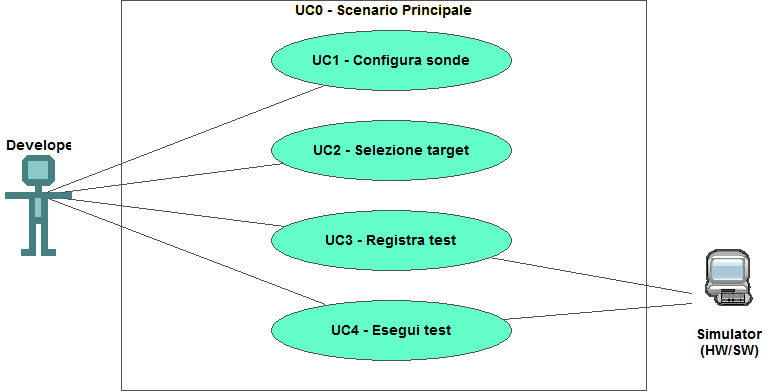
\includegraphics[width=0.9\columnwidth]{usecase/scenario-principale} 
    \caption{Use Case - UC0: Scenario principale}
\end{figure}

\begin{usecase}{0}{Scenario principale}
\usecaseactors{Sviluppatore applicativi}
\usecasepre{Lo sviluppatore è entrato nel plug-in di simulazione all'interno dell'IDE}
\usecasedesc{La finestra di simulazione mette a disposizione i comandi per configurare, registrare o eseguire un test}
\usecasepost{Il sistema è pronto per permettere una nuova interazione}
\label{uc:scenario-principale}
\end{usecase}

\section{Tracciamento dei requisiti}

Da un'attenta analisi dei requisiti e degli use case effettuata sul progetto è stata stilata la tabella che traccia i requisiti in rapporto agli use case.\\
Sono stati individuati diversi tipi di requisiti e si è quindi fatto utilizzo di un codice identificativo per distinguerli.\\
Il codice dei requisiti è così strutturato R(F/Q/V)(N/D/O) dove:
\begin{enumerate}
	\item[R =] requisito
    \item[F =] funzionale
    \item[Q =] qualitativo
    \item[V =] di vincolo
    \item[N =] obbligatorio (necessario)
    \item[D =] desiderabile
    \item[Z =] opzionale
\end{enumerate}
Nelle tabelle \ref{tab:requisiti-funzionali}, \ref{tab:requisiti-qualitativi} e \ref{tab:requisiti-vincolo} sono riassunti i requisiti e il loro tracciamento con gli use case delineati in fase di analisi.

\newpage

\begin{table}%
\caption{Tabella del tracciamento dei requisti funzionali}
\label{tab:requisiti-funzionali}
\begin{tabularx}{\textwidth}{lXl}
\hline\hline
\textbf{Requisito} & \textbf{Descrizione} & \textbf{Use Case}\\
\hline
RFN-1     & L'interfaccia permette di configurare il tipo di sonde del test & UC1 \\
\hline
\end{tabularx}
\end{table}%

\begin{table}%
\caption{Tabella del tracciamento dei requisiti qualitativi}
\label{tab:requisiti-qualitativi}
\begin{tabularx}{\textwidth}{lXl}
\hline\hline
\textbf{Requisito} & \textbf{Descrizione} & \textbf{Use Case}\\
\hline
RQD-1    & Le prestazioni del simulatore hardware deve garantire la giusta esecuzione dei test e non la generazione di falsi negativi & - \\
\hline
\end{tabularx}
\end{table}%

\begin{table}%
\caption{Tabella del tracciamento dei requisiti di vincolo}
\label{tab:requisiti-vincolo}
\begin{tabularx}{\textwidth}{lXl}
\hline\hline
\textbf{Requisito} & \textbf{Descrizione} & \textbf{Use Case}\\
\hline
RVO-1    & La libreria per l'esecuzione dei test automatici deve essere riutilizzabile & - \\
\hline
\end{tabularx}
\end{table}%

    \chapter{Progettazione e codifica}
\label{cap:progettazione-codifica}

\intro{Breve introduzione al capitolo}\\

\section{Tecnologie e strumenti}
\label{sec:tecnologie-strumenti}

Di seguito viene data una panoramica delle tecnologie e strumenti utilizzati.

\subsection*{Tecnologia 1}
Descrizione Tecnologia 1.

\subsection*{Tecnologia 2}
Descrizione Tecnologia 2

\section{Ciclo di vita del software}
\label{sec:ciclo-vita-software}

\section{Progettazione}
\label{sec:progettazione}

\subsubsection{Namespace 1} %**************************
Descrizione namespace 1.

\begin{namespacedesc}
    \classdesc{Classe 1}{Descrizione classe 1}
    \classdesc{Classe 2}{Descrizione classe 2}
\end{namespacedesc}


\section{Design Pattern utilizzati}

\section{Codifica}

    \chapter{Verifica e validazione}
\label{cap:verifica-validazione}

    \chapter{Conclusioni}
\label{cap:conclusioni}

\section{Consuntivo finale}

\section{Raggiungimento degli obiettivi}

\section{Conoscenze acquisite}

\section{Valutazione personale}


    \appendix
    \chapter{Appendice A}

\epigraph{Citazione}{Autore della citazione}


    \backmatter
    \printglossary[type=\acronymtype, title=Acronimi e abbreviazioni, toctitle=Acronimi e abbreviazioni]
    \printglossary[type=main, title=Glossario, toctitle=Glossario]

    \cleardoublepage
\chapter{Bibliografia}

\nocite{*}

% Print book bibliography
%\printbibliography[heading=subbibliography,title={Libri},type=book,resetnumbers=true]
\printbibliography[heading=subbibliography,title={Libri},category=libri,resetnumbers=true]

% Print article bibliography
%\printbibliography[heading=subbibliography,title={Riferimenti bibliografici},type=book,resetnumbers=true]
\printbibliography[heading=subbibliography,title={Articoli},category=articoli,resetnumbers=true]

% Print site bibliography
%\printbibliography[heading=subbibliography,title={Siti web consultati},type=online,resetnumbers=true]
\printbibliography[heading=subbibliography,title={Siti web},category=web,resetnumbers=true]

\end{document}
